\section{Two-by-Two Heckscher-Ohlin Model}

\subsection{Basic environment}

Let's consider an economy with two goods, two factors with endowments $K$ and $L$, where we assume both factors are ``mobile'', can be employed in both sectors.
Output of good $g$ is given by:
\begin{gather*}
    y_g = f^g(K_g, L_g) \quad g = 1,2
\end{gather*}
where $K_g$ and $L_g$ are the endogenous amounts labor and capital in
sector $g$.
$f^g$ is the production function: positive, concave, and increasing in both arguments, and homogeneous of degree 1.

We denote $c_g(w, r) \equiv \text{unit cost function in sector} g$,
then
\begin{gather*}
    c_g(w, r) = \min_{L, K}\{  wL + rK | f^g(L, K) \geq 1\}
\end{gather*}
where $w$ is the wage rate and $r$ is the rental rate of capital.

We then denote $a_{fg} (w,r)$ as the unit demand for factor $f$ in the production of good $g$.
Using the envelope theorem, we can show that:
\begin{gather*}
    a_{fg}(w,r) = \frac{\partial c_g(w,r)}{\partial f} \quad f = K, L
\end{gather*}
We define $A(w,r) \equiv [a_{fg} (w,r)]$ as the matrix of total factor requirements.

\subsection{Equilibrium conditions (I): small open economy}

Like in the Ricardo-Viner Model, we first look at the case of a ``small open
economy'', so there's no need to loot at the good market clearing.

The profit maximization problem of the representative firm in sector $g$ is:
\begin{gather*}
    \max_{L, K} \{ p_g f^g(L, K) - wL - rK \}
\end{gather*}
Taking the FOCs, we can get:
\begin{align*}
    p_g & \leq w a_{Lg}(w,r) + r a_{Kg}(w,r), \text{ for all } g=1,2 \\
    p_g &= w a_{Lg}(w,r) + r a_{Kg}(w,r), \text{ if $g$ is produced in equilibrium.} \tag{Zero-Profit Condition}
\end{align*}
For factor market clearing condition:
\begin{align*}
    L &= y_1 a_{L1}(w,r) + y_2 a_{L2}(w,r) \\
    K &= y_1 a_{K1}(w,r) + y_2 a_{K2}(w,r)
\end{align*}

\subsection{Factor Price Equalization}

\begin{question}
    \

    Can trade in goods be a (perfect) substitute for trade in factors?
\end{question}
First classical result from the HO literature answers by the affirmative.
To establish this result formally, we'll need the following definition:

\begin{definition}[Factor Intensity Reversal]\label{def:FIR}
    \

    Factor Intensity Reversal (FIR) does not occur if:
    \begin{enumerate}
        \item $\frac{a_{L1}(w,r)}{a_{K1}(w,r)} > \frac{a_{L2}(w,r)}{a_{K2}(w,r)}, \forall (w,r)$, or
        \item $\frac{a_{L1}(w,r)}{a_{K1}(w,r)} < \frac{a_{L2}(w,r)}{a_{K2}(w,r)}, \forall (w,r)$
    \end{enumerate}
\end{definition}

\begin{lemma}\label{lem:FIR}
    \
    
    If both goods are produced in equilibrium and FIR does not occur,
    then factor prices $\omega = (w,r)$ are uniquely determined by good
    prices $p = (p_1, p_2)$.
\end{lemma}
\begin{proof}[Proof of Lemma \ref{lem:FIR}]
    \

    If both goods are produced in equilibrium, then we have $A^{\prime} (\omega) \omega = p$.
    By \cite{gale1965}, this equation admits a unique solution if
    $a_{fg}(\omega) > 0$ for all $f,g$, and $\det[A(\omega)] \neq 0$ for all $\omega$,
    which is guaranteed by no FIR.
\end{proof}

By Lemma \ref{lem:FIR}, we know that it's rather the good prices than factor endowments that determine the factor prices.
In a closed economy, good prices and factor endowments are related, but not in a small open economy.
The proof of this lemma has suggested that ``dimensionality'' will be an issue for FIR.

\subsection{Factor Price Insensitivity (FPI): graphical analysis}

Link between no FIR and FPI can be seen graphically:


\tikzset{every picture/.style={line width=0.75pt}} %set default line width to 0.75pt        

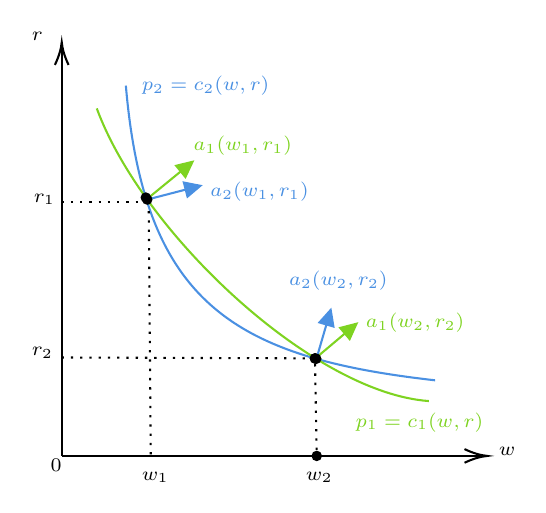
\begin{tikzpicture}[x=0.75pt,y=0.75pt,yscale=-1,xscale=1]
%uncomment if require: \path (0,300); %set diagram left start at 0, and has height of 300

%Straight Lines [id:da6790478314740899] 
\draw    (78.91,229.83) -- (78.91,32.5) ;
\draw [shift={(78.91,30.5)}, rotate = 90] [color={rgb, 255:red, 0; green, 0; blue, 0 }  ][line width=0.75]    (10.93,-3.29) .. controls (6.95,-1.4) and (3.31,-0.3) .. (0,0) .. controls (3.31,0.3) and (6.95,1.4) .. (10.93,3.29)   ;
%Straight Lines [id:da995571939213244] 
\draw    (78.91,229.83) -- (281.91,229.83) ;
\draw [shift={(283.91,229.83)}, rotate = 180] [color={rgb, 255:red, 0; green, 0; blue, 0 }  ][line width=0.75]    (10.93,-3.29) .. controls (6.95,-1.4) and (3.31,-0.3) .. (0,0) .. controls (3.31,0.3) and (6.95,1.4) .. (10.93,3.29)   ;
%Curve Lines [id:da6921719950139332] 
\draw [color={rgb, 255:red, 74; green, 144; blue, 226 }  ,draw opacity=1 ]   (109.8,51.4) .. controls (118.8,156.4) and (161.8,182.4) .. (258.8,193.4) ;
%Straight Lines [id:da07266609586538486] 
\draw  [dash pattern={on 0.84pt off 2.51pt}]  (78.8,107.4) -- (120.8,107.4) ;
%Straight Lines [id:da37631330080024517] 
\draw  [dash pattern={on 0.84pt off 2.51pt}]  (201.8,231.4) -- (200.91,182.83) ;
%Curve Lines [id:da5687671507451815] 
\draw [color={rgb, 255:red, 126; green, 211; blue, 33 }  ,draw opacity=1 ]   (95.8,62.4) .. controls (117.8,122.4) and (199.8,199.4) .. (255.8,203.4) ;
%Straight Lines [id:da802624252602173] 
\draw  [dash pattern={on 0.84pt off 2.51pt}]  (78.8,182.4) -- (200.91,182.83) ;
%Straight Lines [id:da020337326496076558] 
\draw  [dash pattern={on 0.84pt off 2.51pt}]  (120.8,107.4) -- (121.8,229.4) ;
%Straight Lines [id:da4263697333893015] 
\draw [color={rgb, 255:red, 126; green, 211; blue, 33 }  ,draw opacity=1 ]   (120.8,105.4) -- (140.48,89.3) ;
\draw [shift={(142.8,87.4)}, rotate = 140.71] [fill={rgb, 255:red, 126; green, 211; blue, 33 }  ,fill opacity=1 ][line width=0.08]  [draw opacity=0] (8.93,-4.29) -- (0,0) -- (8.93,4.29) -- cycle    ;
%Straight Lines [id:da36565709624802345] 
\draw [color={rgb, 255:red, 74; green, 144; blue, 226 }  ,draw opacity=1 ]   (119.8,106.4) -- (143.9,100.15) ;
\draw [shift={(146.8,99.4)}, rotate = 165.47] [fill={rgb, 255:red, 74; green, 144; blue, 226 }  ,fill opacity=1 ][line width=0.08]  [draw opacity=0] (8.93,-4.29) -- (0,0) -- (8.93,4.29) -- cycle    ;
%Straight Lines [id:da8772767849514311] 
\draw [color={rgb, 255:red, 126; green, 211; blue, 33 }  ,draw opacity=1 ]   (202.8,181.4) -- (219.51,167.33) ;
\draw [shift={(221.8,165.4)}, rotate = 139.9] [fill={rgb, 255:red, 126; green, 211; blue, 33 }  ,fill opacity=1 ][line width=0.08]  [draw opacity=0] (8.93,-4.29) -- (0,0) -- (8.93,4.29) -- cycle    ;
%Straight Lines [id:da9030005673269447] 
\draw [color={rgb, 255:red, 74; green, 144; blue, 226 }  ,draw opacity=1 ]   (201.8,182.4) -- (207.96,161.28) ;
\draw [shift={(208.8,158.4)}, rotate = 106.26] [fill={rgb, 255:red, 74; green, 144; blue, 226 }  ,fill opacity=1 ][line width=0.08]  [draw opacity=0] (8.93,-4.29) -- (0,0) -- (8.93,4.29) -- cycle    ;

% Text Node
\draw (63,176) node [anchor=north west][inner sep=0.75pt]  [font=\scriptsize] [align=left] {$r_{2}$};
% Text Node
\draw (63,24) node [anchor=north west][inner sep=0.75pt]  [font=\scriptsize] [align=left] {$r$};
% Text Node
\draw (288,224) node [anchor=north west][inner sep=0.75pt]  [font=\scriptsize] [align=left] {$w$};
% Text Node
\draw (72,230) node [anchor=north west][inner sep=0.75pt]  [font=\scriptsize] [align=left] {$0$};
% Text Node
\draw (64,102) node [anchor=north west][inner sep=0.75pt]  [font=\scriptsize] [align=left] {$r_{1}$};
% Text Node
\draw (116,236) node [anchor=north west][inner sep=0.75pt]  [font=\scriptsize] [align=left] {$w_{1}$};
% Text Node
\draw (195,236) node [anchor=north west][inner sep=0.75pt]  [font=\scriptsize] [align=left] {$w_{2}$};
% Text Node
\draw (219,207.4) node [anchor=north west][inner sep=0.75pt]  [font=\scriptsize,color={rgb, 255:red, 126; green, 211; blue, 33 }  ,opacity=1 ]  {$p_{1} =c_{1}( w,r)$};
% Text Node
\draw (116,45.4) node [anchor=north west][inner sep=0.75pt]  [font=\scriptsize,color={rgb, 255:red, 74; green, 144; blue, 226 }  ,opacity=1 ]  {$p_{2} =c_{2}( w,r)$};
% Text Node
\draw (141,74.4) node [anchor=north west][inner sep=0.75pt]  [font=\scriptsize,color={rgb, 255:red, 126; green, 211; blue, 33 }  ,opacity=1 ]  {$a_{1}( w_{1} ,r_{1})$};
% Text Node
\draw (149,96.4) node [anchor=north west][inner sep=0.75pt]  [font=\scriptsize,color={rgb, 255:red, 74; green, 144; blue, 226 }  ,opacity=1 ]  {$a_{2}( w_{1} ,r_{1})$};
% Text Node
\draw (224,159.4) node [anchor=north west][inner sep=0.75pt]  [font=\scriptsize,color={rgb, 255:red, 126; green, 211; blue, 33 }  ,opacity=1 ]  {$a_{1}( w_{2} ,r_{2})$};
% Text Node
\draw (187,139.4) node [anchor=north west][inner sep=0.75pt]  [font=\scriptsize,color={rgb, 255:red, 74; green, 144; blue, 226 }  ,opacity=1 ]  {$a_{2}( w_{2} ,r_{2})$};

\draw [fill={rgb, 255:red, 0; green, 0; blue, 0 }  ,fill opacity=1 ]  (201.77, 229.83) circle [x radius= 2, y radius= 2]   ;
\draw [fill={rgb, 255:red, 0; green, 0; blue, 0 }  ,fill opacity=1 ]  (200.91, 182.86) circle [x radius= 2, y radius= 2]   ;
\draw [fill={rgb, 255:red, 0; green, 0; blue, 0 }  ,fill opacity=1 ]  (200.91, 182.83) circle [x radius= 2, y radius= 2]   ;
\draw [fill={rgb, 255:red, 0; green, 0; blue, 0 }  ,fill opacity=1 ]  (119.41, 105.34) circle [x radius= 2, y radius= 2]   ;
\draw [fill={rgb, 255:red, 0; green, 0; blue, 0 }  ,fill opacity=1 ]  (201.53, 183.03) circle [x radius= 2, y radius= 2]   ;
\draw [fill={rgb, 255:red, 0; green, 0; blue, 0 }  ,fill opacity=1 ]  (120.11, 106.32) circle [x radius= 2, y radius= 2]   ;
\end{tikzpicture}

If iso-cost curves cross more than once, then FIR must occur.

\subsection{Factor Price Equalization (FPE) Theorem}

The previous lemma directly implies (Samuelson 1949) that:
\begin{theorem}[FPE Theorem]\label{thm:FPE}
    \

    If two countries produce both goods under free trade with the same technology 
    and FIR does not occur, then they must have the same factor prices.
\end{theorem}

By the FPE theorem, we can regard trade in goods as a `perfect substitution' of trade in factors.
Countries with different factor endowments can sustain same factor
prices through different allocation of factors across sectors.

Assumptions for FPE are stronger than for FPI: we need free trade and
same technology in the two countries...

For next results, we'll maintain assumption that both goods are
produced in equilibrium, but won't need free trade and same technology.

\subsection{Stolper-Samuelson Theorem}

\begin{theorem}[Stolper-Samuelson Theorem]\label{thm:SS}
    \

    An increase in the relative price of a good will increase the real return
    to the factor used intensively in that good, and reduce the real return to the other factor.
\end{theorem}

\begin{proof}[Proof of Theorem \ref{thm:SS}]
    \

    W.l.o.g. we assume that:
    \begin{enumerate}
        \item $\frac{a_{L1}(\omega)}{a_{K1}(\omega)} > \frac{a_{L2}(\omega)}{a_{K2}(\omega)}$, meaning that good 1 is labor-intensive and good 2 is capital-intensive.
        \item $\hat{p}_2 > \hat{p}_1$, meaning that the price of good 2 increases relative to the price of good 1.
    \end{enumerate}
    As we know that $p_g = w a_{Lg} + r a_{Kg}$, we differentiate on both sides:
    \begin{gather*}
        d p_g = a_{Lg} dw + a_{Kg} dr \quad g = 1,2 \\
        \Rightarrow \hat{p}_g = \frac{d p_g}{p_g} = \frac{a_{Lg}}{w a_{Lg} + r a_{Kg}} d w + \frac{a_{Kg}}{w a_{Lg} + r a_{Kg}} d r = \theta_{Lg} \hat{w} + (1-\theta_{Lg} ) \hat{r} \\
        \text{where } \theta_{Lg} =  \frac{w a_{Lg}}{C_g(\omega)}
    \end{gather*}
    As we assume $\frac{a_{L1}}{a_{K1}} > \frac{a_{L2}}{a_{K2}}$, $\theta_{L1} > \theta_{L2}$,
    thus $\hat{p}_2 > \hat{p}_1$ only requires $\hat{r} > \hat{w}$, and we could get:
    \begin{gather*}
        \hat{r} > \hat{p}_2 > \hat{p}_1 > \hat{w}
    \end{gather*}
    which is also the `magnification effect'.
\end{proof}

The Stolper-Samuelson theorem predict both winners and losers from change in relative prices.
Like FPI and FPE \ref{thm:FPE}, SS entirely comes from zero-profit condition (+ no
joint production).

Like FPI and FPE, sharpness of the result hinges on `dimensionality'.
In the empirical literature, people often talk about ``Stolper-Samuelson
effects'' whenever looking at changes in relative factor prices (though
changes in relative good prices are rarely observed).

\subsection{Stolper-Samuelson (1941) Theorem: graphical analysis}



\tikzset{every picture/.style={line width=0.75pt}} %set default line width to 0.75pt        

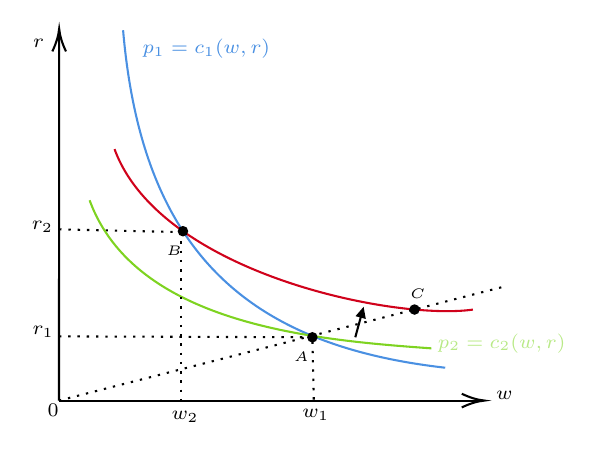
\begin{tikzpicture}[x=0.75pt,y=0.75pt,yscale=-1,xscale=1]
%uncomment if require: \path (0,300); %set diagram left start at 0, and has height of 300

%Straight Lines [id:da7262511276836261] 
\draw    (98.91,249.83) -- (99,72.67) ;
\draw [shift={(99,70.67)}, rotate = 90.03] [color={rgb, 255:red, 0; green, 0; blue, 0 }  ][line width=0.75]    (10.93,-3.29) .. controls (6.95,-1.4) and (3.31,-0.3) .. (0,0) .. controls (3.31,0.3) and (6.95,1.4) .. (10.93,3.29)   ;
%Straight Lines [id:da651779350603288] 
\draw    (98.91,249.83) -- (301.91,249.83) ;
\draw [shift={(303.91,249.83)}, rotate = 180] [color={rgb, 255:red, 0; green, 0; blue, 0 }  ][line width=0.75]    (10.93,-3.29) .. controls (6.95,-1.4) and (3.31,-0.3) .. (0,0) .. controls (3.31,0.3) and (6.95,1.4) .. (10.93,3.29)   ;
%Curve Lines [id:da13355067232797913] 
\draw [color={rgb, 255:red, 74; green, 144; blue, 226 }  ,draw opacity=1 ]   (129.8,71.4) .. controls (138.8,176.4) and (188,223) .. (285,234) ;
%Straight Lines [id:da36347828521645387] 
\draw  [dash pattern={on 0.84pt off 2.51pt}]  (99,167.33) -- (157.67,168.67) ;
%Straight Lines [id:da891510439583168] 
\draw  [dash pattern={on 0.84pt off 2.51pt}]  (221.67,249.33) -- (221,219.33) ;
%Curve Lines [id:da20193881286275817] 
\draw [color={rgb, 255:red, 126; green, 211; blue, 33 }  ,draw opacity=1 ]   (113.67,153.33) .. controls (135.67,213.33) and (222.33,220.67) .. (278.33,224.67) ;
%Straight Lines [id:da30847342006781875] 
\draw  [dash pattern={on 0.84pt off 2.51pt}]  (98.89,218.9) -- (221,219.33) ;
%Straight Lines [id:da2497408700390059] 
\draw  [dash pattern={on 0.84pt off 2.51pt}]  (157.67,168.67) -- (157.67,249.33) ;
%Curve Lines [id:da2864338426884703] 
\draw [color={rgb, 255:red, 208; green, 2; blue, 27 }  ,draw opacity=1 ]   (125.67,128.67) .. controls (147.67,188.67) and (261,211.33) .. (298.33,206) ;
%Straight Lines [id:da7278489062710455] 
\draw  [dash pattern={on 0.84pt off 2.51pt}]  (98.91,249.83) -- (314.33,194.67) ;
%Straight Lines [id:da27901197251833265] 
\draw    (241.67,219.33) -- (244.88,207.56) ;
\draw [shift={(245.67,204.67)}, rotate = 105.26] [fill={rgb, 255:red, 0; green, 0; blue, 0 }  ][line width=0.08]  [draw opacity=0] (5.36,-2.57) -- (0,0) -- (5.36,2.57) -- cycle    ;

% Text Node
\draw (84.33,162) node [anchor=north west][inner sep=0.75pt]  [font=\scriptsize] [align=left] {$r_{2}$};
% Text Node
\draw (85,74) node [anchor=north west][inner sep=0.75pt]  [font=\scriptsize] [align=left] {$r$};
% Text Node
\draw (308,244) node [anchor=north west][inner sep=0.75pt]  [font=\scriptsize] [align=left] {$w$};
% Text Node
\draw (92,250) node [anchor=north west][inner sep=0.75pt]  [font=\scriptsize] [align=left] {$0$};
% Text Node
\draw (84.67,212.67) node [anchor=north west][inner sep=0.75pt]  [font=\scriptsize] [align=left] {$r_{1}$};
% Text Node
\draw (214.67,252.67) node [anchor=north west][inner sep=0.75pt]  [font=\scriptsize] [align=left] {$w_{1}$};
% Text Node
\draw (151.67,253.33) node [anchor=north west][inner sep=0.75pt]  [font=\scriptsize] [align=left] {$w_{2}$};
% Text Node
\draw (280,216.07) node [anchor=north west][inner sep=0.75pt]  [font=\scriptsize,color={rgb, 255:red, 184; green, 233; blue, 134 }  ,opacity=1 ]  {$p_{2} =c_{2}( w,r)$};
% Text Node
\draw (137.67,74.07) node [anchor=north west][inner sep=0.75pt]  [font=\scriptsize,color={rgb, 255:red, 74; green, 144; blue, 226 }  ,opacity=1 ]  {$p_{1} =c_{1}( w,r)$};
% Text Node
\draw (149.33,174.07) node [anchor=north west][inner sep=0.75pt]  [font=\tiny]  {$B$};
% Text Node
\draw (210.67,224.73) node [anchor=north west][inner sep=0.75pt]  [font=\tiny]  {$A$};
% Text Node
\draw (266.67,194.73) node [anchor=north west][inner sep=0.75pt]  [font=\tiny]  {$C$};

\draw [fill={rgb, 255:red, 0; green, 0; blue, 0 }  ,fill opacity=1 ]  (221, 219.33) circle [x radius= 2, y radius= 2]   ;
\draw [fill={rgb, 255:red, 0; green, 0; blue, 0 }  ,fill opacity=1 ]  (158.65, 168.23) circle [x radius= 2, y radius= 2]   ;
\draw [fill={rgb, 255:red, 0; green, 0; blue, 0 }  ,fill opacity=1 ]  (270.21, 205.97) circle [x radius= 2, y radius= 2]   ;
\end{tikzpicture}

Like for FPI and FPE, all economic intuition could be gained by
looking at the simpler Leontieff case:
In the general case, iso-cost curves are not straight lines, but under no
FIR, same logic applies.

\subsection{Rybczynski (1965) Theorem}
Previous results have focused on the implication of zero profit
condition, the factor prices. We now turn our attention to the implication of factor market
clearing, the factor allocation.

\begin{theorem}[Rybczynski Theorem]\label{thm:Ryb}
    \

    An increase in factor endowment will increase the output of the industry using it intensively,
    and decrease the output of the other industry.
\end{theorem}

\begin{proof}[Proof of ]
    \

    W.l.o.g. we assume that:
    \begin{enumerate}
        \item $\frac{a_{L1}}{a_{K1}} > \frac{a_{L2}}{a_{K2}}$, meaning that good 1 is labor-intensive and good 2 is capital-intensive.
        \item $\hat{K} > \hat{L}$, meaning that the endowment of capital increases relative to the endowment of labor.
    \end{enumerate}
    We know that $L = y_1 a_{L1} + y_2 a_{L2}$, thus we can differentiate on both sides:
    \begin{gather*}
        d L = a_{L1} d y_1 + a_{L2} d y_2 \\
        \Rightarrow \hat{L} = \frac{d L}{L} = \frac{a_{L1}}{L} d y_1 + \frac{a_{L2}}{L} d y_2 = \lambda_{L1} \hat{y}_1 + (1-\lambda_{L1}) \hat{y}_2
    \end{gather*}
    Similarly, we can get:
    \begin{gather*}
        \hat{K} = \frac{d K}{K} = \frac{a_{K1}}{K} d y_1 + \frac{a_{K2}}{K} d y_2 = \lambda_{K1} \hat{y}_1 + (1-\lambda_{K1}) \hat{y}_2
    \end{gather*}
    where $\lambda_{L1} = \frac{a_{L1} y_1}{L}$ and $\lambda_{K1} = \frac{a_{K1} y_1}{K}$.
    As we assume $\frac{a_{L1}}{a_{K1}} > \frac{a_{L2}}{a_{K2}}$,  we know that $\lambda_{L1} > \lambda_{K1}$.
    So $\hat{K} > \hat{L}$ only requires $\hat{y}_2 > \hat{y}_1$, and we could get:
    \begin{gather*}
        \hat{y}_2 > \hat{K} > \hat{L} > \hat{y}_1.
    \end{gather*}
\end{proof}

Like for FPI and FPE Theorems, hte prices $(p_1, p_2)$ are exogenously given,
so the factor prices and factor requirements are not affected by changes factor endowments.

Empirically, Rybczynski Theorem suggests that impact of immigration
may be very different in closed vs. open economy

Like for SS Theorem, we have a ``magnification effect''.

Like for FPI, FPE, and SS Theorems, sharpness of the result
hinges on ``dimensionality''.

\subsection{Rybczynski Theorem: graphical analysis}

Since good prices are fixed, it is as if we were in Leontieff case.



\tikzset{every picture/.style={line width=0.75pt}} %set default line width to 0.75pt        

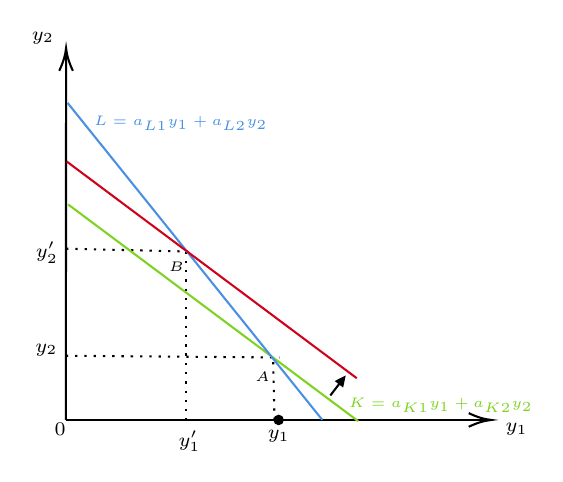
\begin{tikzpicture}[x=0.75pt,y=0.75pt,yscale=-1,xscale=1]
%uncomment if require: \path (0,300); %set diagram left start at 0, and has height of 300

%Straight Lines [id:da16249243577419226] 
\draw    (98.91,249.83) -- (99,72.67) ;
\draw [shift={(99,70.67)}, rotate = 90.03] [color={rgb, 255:red, 0; green, 0; blue, 0 }  ][line width=0.75]    (10.93,-3.29) .. controls (6.95,-1.4) and (3.31,-0.3) .. (0,0) .. controls (3.31,0.3) and (6.95,1.4) .. (10.93,3.29)   ;
%Straight Lines [id:da9440179025397044] 
\draw    (98.91,249.83) -- (301.91,249.83) ;
\draw [shift={(303.91,249.83)}, rotate = 180] [color={rgb, 255:red, 0; green, 0; blue, 0 }  ][line width=0.75]    (10.93,-3.29) .. controls (6.95,-1.4) and (3.31,-0.3) .. (0,0) .. controls (3.31,0.3) and (6.95,1.4) .. (10.93,3.29)   ;
%Straight Lines [id:da9474972780686752] 
\draw  [dash pattern={on 0.84pt off 2.51pt}]  (99,167.33) -- (157.67,168.67) ;
%Straight Lines [id:da37522216818053933] 
\draw  [dash pattern={on 0.84pt off 2.51pt}]  (199.41,249.83) -- (198.75,219.83) ;
%Straight Lines [id:da03911186399497246] 
\draw  [dash pattern={on 0.84pt off 2.51pt}]  (98.89,218.9) -- (201.73,219.73) ;
%Straight Lines [id:da1861077956660001] 
\draw  [dash pattern={on 0.84pt off 2.51pt}]  (156.67,168.67) -- (156.67,249.33) ;
%Straight Lines [id:da26470960694675294] 
\draw    (226.33,238) -- (231.9,230.78) ;
\draw [shift={(233.73,228.4)}, rotate = 127.63] [fill={rgb, 255:red, 0; green, 0; blue, 0 }  ][line width=0.08]  [draw opacity=0] (5.36,-2.57) -- (0,0) -- (5.36,2.57) -- cycle    ;
%Straight Lines [id:da006187412728739461] 
\draw [color={rgb, 255:red, 126; green, 211; blue, 33 }  ,draw opacity=1 ]   (100,146) -- (239.73,250.4) ;
%Straight Lines [id:da16115080230280587] 
\draw [color={rgb, 255:red, 74; green, 144; blue, 226 }  ,draw opacity=1 ]   (99.73,97.07) -- (222.4,249.73) ;
%Straight Lines [id:da1891620825225372] 
\draw [color={rgb, 255:red, 208; green, 2; blue, 27 }  ,draw opacity=1 ]   (99.33,125.33) -- (239.07,229.73) ;

% Text Node
\draw (81,61.33) node [anchor=north west][inner sep=0.75pt]  [font=\scriptsize] [align=left] {$y_{2}$};
% Text Node
\draw (309.33,250) node [anchor=north west][inner sep=0.75pt]  [font=\scriptsize] [align=left] {$y_{1}$};
% Text Node
\draw (92,250) node [anchor=north west][inner sep=0.75pt]  [font=\scriptsize] [align=left] {$0$};
% Text Node
\draw (194.67,253.33) node [anchor=north west][inner sep=0.75pt]  [font=\scriptsize] [align=left] {$y_{1}$};
% Text Node
\draw (151.67,253.33) node [anchor=north west][inner sep=0.75pt]  [font=\scriptsize] [align=left] {$y_{1}^{\prime} $};
% Text Node
\draw (111,102.07) node [anchor=north west][inner sep=0.75pt]  [font=\tiny,color={rgb, 255:red, 74; green, 144; blue, 226 }  ,opacity=1 ]  {$L=a_{L1} y_{1} +a_{L2} y_{2}$};
% Text Node
\draw (147,172.07) node [anchor=north west][inner sep=0.75pt]  [font=\tiny]  {$B$};
% Text Node
\draw (188.67,225.4) node [anchor=north west][inner sep=0.75pt]  [font=\tiny]  {$A$};
% Text Node
\draw (82.67,211.67) node [anchor=north west][inner sep=0.75pt]  [font=\scriptsize] [align=left] {$y_{2}$};
% Text Node
\draw (83.00,162.33) node [anchor=north west][inner sep=0.75pt]  [font=\scriptsize] [align=left] {$y_{2}^{\prime} $};
% Text Node
\draw (233.73,237.8) node [anchor=north west][inner sep=0.75pt]  [font=\tiny,color={rgb, 255:red, 126; green, 211; blue, 33 }  ,opacity=1 ]  {$K=a_{K1} y_{1} +a_{K2} y_{2}$};

\draw [fill={rgb, 255:red, 0; green, 0; blue, 0 }  ,fill opacity=1 ]  (201.41, 249.83) circle [x radius= 2, y radius= 2]   ;
\end{tikzpicture}

\subsection{Constructing the Edgeworth Box Diagram}
